\section{A constructive witness with a stronger alternative}\label{sec:study}
The new companion makes the connection between production, choice, cash and succession executable in a finite analytical model. Its inputs are deliberately authored. It does not discover an unknown technology or estimate market demand. The substantive question is whether a productive change and a voluntary contract can jointly make an accepted outcome reachable, and whether that result survives composed purchases and a capable conventional comparison.

\subsection{The same outcome and the same total process cost}
There are two separately useful services, $A$ and $B$. Their values to the illustrative buyer are $7$, $7$ and $14$ for $A\cup B$. The outside option is zero. The buyer has sufficient budget for the two purchases, may refuse each stage, and buys only for strictly positive incremental utility. The offered component prices are $6$ and $6$; an advertised joint quote of $13$ therefore closes to $12$ when both components can be purchased. All amounts in this section are abstract units.

The required final accepted output is identical across four production and contracting arrangements. Their declared complete process cost is also identical: $9$. Ordinary monolithic production incurs that cost before completion. Ordinary staged production incurs $7$ before its first useful accepted output and $2$ afterward. A supplied connector costs $2$ to construct and changes the productive path to an initial stage costing $3$, followed by a continuation costing $4$. The stage envelopes include their declared acceptance work. A final-payment contract collects only after both outputs; a staged contract collects $6$ after each independently accepted, useful output.

\begin{table}[ht]
\small\centering
\begin{tabularx}{\linewidth}{@{}Yrr@{}}\toprule
Construction and payment arrangement & Total process cost & Minimum opening cash\\\midrule
Ordinary production, final payment & 9 & 9\\
Staged payment alone & 9 & 7\\
Connector alone, final payment & 9 & 9\\
Connector with useful verified staging & 9 & \textbf{5}\\\bottomrule
\end{tabularx}
\caption{A conditional liquidity complementarity. The final accepted outcome and total declared process cost are unchanged. The last row changes both the productive path and the timing of earned receipts.}
\label{tab:stages}
\end{table}

At opening cash $6$, neither isolated change makes the complete route executable. The joint construction does. It incurs the connector and first-stage expenses, delivers and verifies a useful output, collects the earned payment and funds the continuation. The exact cash path is
\begin{equation}
6\ \xrightarrow{-2}\ 4\ \xrightarrow{-3}\ 1
\ \xrightarrow{+6}\ 7\ \xrightarrow{-4}\ 3
\ \xrightarrow{+6}\ 9.
\label{eq:trace}
\end{equation}
Receipts are $12$ and declared process costs are $9$, leaving a three-unit modeled operating surplus. The first payment is earned for a completed, independently useful output. It is not a refundable deposit silently treated as working capital. The buyer gains one unit of value at each stage and can refuse. Given the stipulated enforceable fixed price and accepted first stage, the seller also prefers the continuation: it incurs four more units to collect six. The example assumes reliable execution and the declared acceptance semantics; it does not establish them for a physical service.

\begin{figure}[ht]
\centering
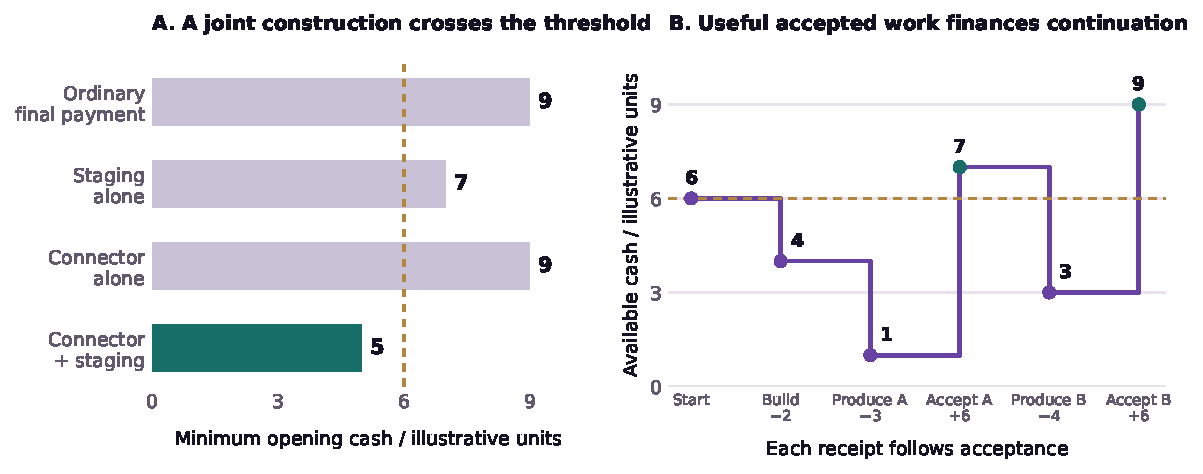
\includegraphics[width=\linewidth]{figures/construction.pdf}
\caption{Exact analytical witness. Left: the opening-capital threshold of each complete route. Right: the joint route uses receipts only after a useful stage is accepted. The dashed horizontal line is the available starting capital, not a universal capital restriction.}
\label{fig:construction}
\end{figure}

The constructive change is therefore specific. It creates a useful intermediate output early enough for voluntary earned payment to finance continuation. Staging a promise without such an output would not satisfy the model. Merely relabeling a payment would not repair the ordinary path's seven-unit initial requirement. The connector's productive effect is a supplied hypothesis in this witness, not a technology autonomously discovered by the companion.

\subsection{Additional burdens remain visible}
The nine-unit envelope is an analytical process specification, not a measured complete commercial invoice. Let $h\ge0$ represent an additional common lifecycle burden, paid before the process begins. It can stand for otherwise unmodeled discovery, acquisition, administration, financing or residual obligations. The joint route then requires $5+h$ opening units and leaves surplus $3-h$. At the fixed opening balance of $6$, it can execute only when $h\le1$; its surplus is positive only when $h<3$.

This sensitivity prevents an included computation from becoming an assertion of free economic resources. If an additional burden occurs later, its actual timing belongs in the cash plan. If the delivery can fail or incur refunds, the corresponding branch and protections must be modeled. The fixed deterministic trace establishes only its declared execution. It is not a native enterprise account and does not overwrite any laboratory financial history.

\subsection{The conventional constructor has the same freedom}
The complete conventional control can choose every supplied production route and every allowed contract. It finds the same feasible joint arrangement at opening cash $6$. The constructive result is real within the model; an inventor-superiority result does not follow.

Changing capital also changes the best choice. At $7$, ordinary staging becomes feasible and can tie the three-unit surplus without the new connector. At $9$, an ordinary final-only route can offer only the complete bundle for $13$. With value $14$, the buyer strictly prefers that purchase to refusal; the four-unit surplus exceeds the staged route's three. This pure-bundle offer does not advertise the cheaper component purchases, and it receives no early stage payment. It is a legitimate, stronger complete alternative when the initial cost can be funded.

The companion evaluates these route and price choices within a declared finite domain. No route receives hypothetical credit. A separately specified, voluntarily supplied financing contract could change the ranking, with its cost and repayment included. The calculation therefore identifies where a joint construction helps under a resource boundary; it does not establish that the selected capital is globally optimal or that the joint route is always preferable.

There is also an instructive tie in the original menu: values $7,7,14$ and posted prices $6,6,13$ give single-purchase utilities $1,1,1$. One cannot infer that a single-purchase buyer pays $13$. The cart yields utility $2$ and payment $12$. The study preserves refusal and indifference rules explicitly rather than selecting the buyer action that makes the seller's claim look best.

\subsection{A strategic omission can invent a fictitious successor}
After the executed joint route, cash is $9$. A projection that substitutes the advertised joint quote of $13$ for the actual aggregate receipts of $12$ would report cash $10$. It would therefore appear to fund a successor requiring ten upfront units, even though the actual route is one unit short. This is a deliberately authored illustration of Equation~\ref{eq:leakage}; the $13$ receipt is a naive quote-based projection, not a rational single-purchase result for this menu.

Profit and cash remain different. The first route's three-unit surplus does not mean that only three units of cash exist. A four-unit successor is affordable from the actual nine-unit balance, subject to the stated zero remaining obligations. That funding would use a mixture of opening capital and earnings unless a separate attribution establishes otherwise. Protecting the entire initial capital solely to manufacture a stronger enabling result would change the experiment.

On a subsequent use, the retained connector avoids its two-unit reconstruction cost. The fresh process costs $7$ and can leave surplus $5$ at the same twelve-unit receipts. Rebuilding costs $9$ and leaves $3$. Ordinary reuse of identical connector content ties the retained method. This is a fixed-menu, fixed-schedule inheritance comparison. The improvement is attributable to the available artifact, not to a demonstrated improvement of the invention procedure; the first construction cost remains in the two-episode history.

The stronger adaptive continuation should also be used. On a fresh task whose offer need not retain the earlier component commitments, the retained connector can support final-only production costing $7$ and a pure-bundle receipt of $13$. The first episode's closing cash of $9$ funds that path. The second surplus is then $6$, total two-episode surplus is $9$, and cash ends at $15$. An ordinary controller with the same asset and choices ties. Fixing the earlier staged contract indefinitely would miss a legitimate improvement made possible by the changed state.

\subsection{Exact verification and its domain}
The companion enumerates 2,187 three-service price menus, corresponding to seven nonempty service sets with prices in $\{1,2,3\}$. The union-graph calculation agrees with independent enumeration of 279,936 carts and all 413,343 buyer-and-budget comparisons. It also checks 139,968 subadditivity inequalities and 15,309 coordinatewise price increases, along with contractivity and idempotence. These are exhaustive finite checks, not independent market observations.

A separate two-service search considers 4,096 menus, with each price either absent or in $\{0,\ldots,14\}$. It preserves explicit best responses, budgets and non-entry. Allowing carts raises seller receipts in 341 menus, lowers them in 91 and leaves them unchanged in 3,664. The effective joint quote is lower than the posted joint quote in 560 menus. Thus the fixed-choice regret result does not imply that adding buyer options always lowers actual revenue: the selected outcome can change. Both complete pricing methods identify the pure-bundle-only price $13$ as a revenue optimum in this one-shot domain.

The separate joint price-and-route search evaluates 480 contracts plus non-entry. At opening cash $6$, 126 contracts satisfy the modeled buyer participation conditions, 28 are financeable and six have positive surplus. The best feasible arrangement uses the connector and staged prices $(6,6)$, producing surplus $3$. At opening cash $9$, ordinary pure bundling produces surplus $4$. The independent conventional control has every same choice and ties both optima. Twenty-four focused tests pass, including false equivalence, unsupported unions, exact budgets, buyer ties, financial timing, overhead and the stronger successor continuation.

These finite calculations establish exact agreement and conditional optima within their supplied domains. They are not estimates of real behavior, a statistical confirmation set, or evidence that the program invented the service primitives. The source includes the protocol, executable companion, independent cart oracle, focused regressions, deterministic result file and the plotted trace. Appendix~\ref{app:proofs} states the mathematical assumptions, and the reproduction guide explains how to regenerate the checks and paper.
